\chapter{INTRODUCTION}



In broadest terms, this dissertation investigates ``pairing up'' problems.  Assigning workers to jobs, putting students into cooperative pairs, scheduling processes to machines, and choosing efficient locations for building bridges between roads are all examples of this sort of problem.  We look at special kinds of pairing schemes that have certain interconnectedness properties, and how they can be accomplished under various restrictions in diverse circumstances.  

When we model these scenarios with graphs, the type of pairing we are interested in will be called a connected matching.  While gaining insight into practical issues such as the ones listed above is a worthy goal on its own, we will see that detecting connected matchings in graphs is a rich and complex computational task.  Furthermore, in certain families of graphs, the existence of large connected matchings is equivalent to Hadwiger's conjecture, a famous open problem in graph theory.  
  
		

The objective in this study is to carry forward the theory of connected matchings in both the computational and structural areas.  We aim to further flesh out the complexity of detecting connected matchings, determining with greater specificity the classes of graphs for which connected matching problems are tractable.  We also present progress on a conjecture related to the existence of large connected matchings in graphs with independence number 2.  We will also consider real world problems to which we apply our findings.



In the remainder of this chapter, we walk through the basic graph theoretic ideas employed in this dissertation, and introduce some new ideas that clarify later explanations.  Next, we will introduce the extremal problem of connected matchings and place it in a theoretical context.  In Chapter 3, we will present recent progress and original work on a version of that extremal problem.  In Chapters 4 and 5, we will explore the computational issue of detecting connected matchings in some special families of graphs, and cite examples of optimization problems that can make use of these results.  Finally, we will take a look at problems that are tangential to our main subject, but too appealing to be left behind.     

\section{Background}
	

Formally speaking, a {\it finite simple graph} \index{Graph} $G = (V(G), E(G))$ consists of a set $V(G)$ called the {\it vertex set} \index{Vertex} and a set $E(G)$ of two element subsets of $V(G)$ called the {\it edge set}\index{Edge}.  We think of a graph as a collection of vertices, some of which are joined by edges.  Graphs are typically used to model systems with a connectedness relation, as in the following examples:
	\begin{itemize}
		\item A collection of people is modeled with a vertex set and an edge is placed between pairs of vertices corresponding to pairs of people who are friendly with each other (a {\it social network} graph).
		\item A collection of computers is modeled with a vertex set and an edge is placed between pairs of vertices corresponding to pairs of computers with a physical network cable between them (a {\it computer network} graph).
		\item The courses in a mathematics department are modeled with vertices. An edge is placed between them if their meeting times overlap (a {\it scheduling} graph).
	\end{itemize}
We use a shortened notation for edges.  If edge $e$ in a graph $G$ is the set containing vertices $u$ and $v$, we write $e = uv$.  The {\it complement}\index{graph complement} of a graph $G$, denoted $\overline{G}$, is the graph on the same vertex set as $G$ in which the edge $uv \in E(\overline{G})$ if and only if $uv \notin E(G)$.

\subsection{Matchings and connected matchings}
An edge $e$ of a graph is said to be {\it incident} to each of its endpoints.  A vertex $v$ is {\it saturated} or {\it covered} by any collection of edges containing an edge incident to $v$.
A {\it matching} \index{Matching}in a graph is a collection of disjoint edges.  A {\it perfect} matching \index{Matching!perfect}is a matching that covers every vertex in the graph exactly once.  Each vertex covered by a matching is ``matched'' unambiguously to one other vertex by the matching edge that touches it.  

A powerful theoretical tool for proving the existence of matchings is {\it Hall's condition}\index{Hall's condition}.  For a set $S$ of vertices in a graph $G$, let $N(S)$ be the {\it open neighborhood} of $S$, that is, the set of vertices in $V(G)-S$ that are adjacent to a vertex from $S$.  Hall's condition, which can be proven by induction, states that if $S$ has the property that for every subgraph $T \subseteq S$, $|N(T) \cap V(G)-S| \geq |T|$, then there is a matching in $G$ from $S$ to $G-S$ that saturates $S$.  We will apply Hall's condition several times in this study. 

Matchings in graphs are used to model pairings.  Consider a graph with one subset of vertices representing jobs and another representing workers.  Place an edge between a job and a worker if that worker is trained to perform that job.  If each worker performs one job at a time, and each job needs only one worker, then a feasible assignment of jobs to workers is modeled by a matching.

A pair of disjoint edges $e = uv$ and $f = xy$ in a graph $G$ is {\it separable}\index{Separable edges} if and only if none of the edges $ux, uy, vx, vy$ are present in $G$.  A pair of edges that are not separable is called {\it neighborly}\index{Neighborly edges}.  A graph is called separable if and only if it has a separable pair ofedges.  Figure \ref{separable} exhibits the ways in which a pair of edges in a graph may be separable or neighborly.  

	\begin{figure}
	\begin{center}
		\begin{tikzpicture}[thick,scale=0.75]

	\coordinate (a0) at (0:0);
	\coordinate (a1) at (180:1);
	\coordinate (a3) at (-109:3);
	\coordinate (a2) at (0:1);
	\coordinate (a4) at (-71:3);
	\coordinate (text) at (-90:4);
	\coordinate (b2) at (30:3);

	\draw (a0)-- node[lblvertex] {e}(a3);
	\draw (a0)-- node[lblvertex] {f}(a4);

	\draw (a0) node {};	
	\draw (text) node[words] {neighborly};
	\draw (a3) node {};
	\draw (a4) node {};
	
\end{tikzpicture}
\hspace{2cm}
		\begin{tikzpicture}[thick,scale=0.5]

	\coordinate (a0) at (0:0);
	\coordinate (a1) at (180:1);
	\coordinate (a3) at (-109:3);
	\coordinate (a2) at (0:1);
	\coordinate (a4) at (-71:3);
	\coordinate (text) at (-90:4);
	\coordinate (b2) at (30:3);

	\draw (a1)-- node[lblvertex] {e}(a3);
	\draw (a2)-- node[lblvertex] {f}(a4);
	\draw (a1)--(a4);
	\draw (a1) node[]{};
	\draw (a2) node[]{};
	\draw (a3) node[]{};
	\draw (a4) node[]{};
	\draw (text) node[words] {neighborly};
\end{tikzpicture}
\hspace{2cm}
		\begin{tikzpicture}[thick,scale=0.75]

	\coordinate (a0) at (0:0);
	\coordinate (a1) at (180:1);
	\coordinate (a3) at (-109:3);
	\coordinate (a2) at (0:1);
	\coordinate (a4) at (-71:3);
	\coordinate (b1) at (150:3);
	\coordinate (text) at (-90:4);

	\draw (a1)-- node[lblvertex] {e}(a3);
	\draw (a2)-- node[lblvertex] {f}(a4);
	\draw (a1) node[]{};
	\draw (a2) node[]{};
	\draw (a3) node[]{};
	\draw (a4) node[]{};
	\draw (text) node[words] {separable};
	
\end{tikzpicture}

		\label{separable}
		\caption{Neighborly and separable pairs of edges.}
	\end{center}
	\end{figure}
A {\it connected matching} \index{Matching!connected}in a graph $G$ is a matching $M$ with the additional property that no two edges of $M$ are separable in $G$.  We use this property to model various ``matching-type'' problems with extra requirements.   
  
\subsection{Graph coloring}
Suppose we have a graph $G = (V, E)$.  If we take a subset $V'$ of $V$ and subset $E'$ of $E$ so that every $e$ in $E'$ is a subset of $V'$, then the graph $G' = (V',E')$ is called a {\it subgraph} of $G$.  Intuitively, we create a subgraph by selecting  vertices from a graph, and then choosing to include or exclude edges from the original graph whose endpoints are among the vertices we have selected.  An edge that has both endpoints in a set $S$ of vertices is said to be \textit{induced} \index{induced edge}by $S$.  The subgraph created by choosing a set $S$ of vertices and all edges induced by $S$ is called the subgraph of $G$ induced by $S$\index{induced subgraph}, denoted $G[S]$.
 
A set of vertices in a graph is called {\it independent}\index{Vertex!independent sets of} if it induces a graph with no edges.  Let $\alpha(G)$ denote the size of the largest independent vertex set of $G$, called the {\it independence number}\index{independence number} of a graph $G$.  

Consider the scheduling graph we introduced earlier in this section\index{scheduling graph}.  If two classes are in meetings at the same time at any point during the week, the corresponding vertices are joined by an edge.  Each independent set therefore represents a collection of courses that do not overlap in time. Hence, a collection of courses we could feasibly assign to a single instructor corresponds to an independent set of vertices in the scheduling graph.  We therefore model the task of assigning courses to instructors by partitioning the vertices of the scheduling graph into independent sets.

Another way of looking at a partition of this kind is as a {\it proper vertex coloring}\index{proper vertex coloring}.  Suppose we give each instructor a color, and visualize the scheduling graph with each vertex colored according to the instructor assigned to the corresponding course.  If the assignment is feasible, then no pair of adjacent vertices has the same color assigned to each.  Formally, we define a proper vertex coloring as a partition $\mathcal{C} = \{C_1, C_2, \ldots, C_k\}$ of the vertex set of a graph $G$ with the property that each color class $C_i$ is an independent set.

A natural question arises in the scheduling graph model. How many instructors are needed to teach a certain collection of courses?  In general, given a graph $G$, how many colors are needed to properly color its vertices?   
The minimum number of colors needed to properly color a graph $G$ is called the {\it chromatic number}\index{Chromatic number} of $G$, denoted $\chi(G)$.  For instance, a collection of three mutually adjacent vertices clearly requires three different colors in a proper coloring.  However, a sequence of vertices each of which is adjacent to the precedent and antecedent vertices (a {\it path} graph\index{path}) requires only two colors no matter how many vertices are used.   A particularly interesting class of graphs are those with chromatic number two, called {\it bipartite graphs}\index{bipartite graph}.  We denote a bipartite graph $G$ as $(A,B; E)$ where $E$ is the edge set and $A$ and $B$ are the {\it partite sets}\index{partite set}, i.e., the independent sets in a particular proper coloring of $G$.

\subsection{Perfect graphs}

The complementary notion of independence is {\it completeness}\index{Complete graph|see{clique}}.  If a subset $S$ of vertices in a graph $G$ induces all possible edges between vertices of $S$, we say $S$ induces a {\it complete graph} or a {\it clique}\index{Clique}.  For the complete graph on $n$ vertices, we use the notation $K_n$.  The size of the largest clique contained in $G$ is the {\it clique number}, denoted $\omega(G)$\index{Clique number}.

It's not hard to see that if a graph contains a clique on $k$ vertices, then a proper coloring will require at least $k$ colors.  Each vertex of the clique is adjacent to all the others, and thus requires its own color.   However, it is not the case that a graph must contain a clique on $k$ vertices to require $k$ colors for proper coloring.  Consider a graph on five vertices $v_1, v_2, v_3, v_4,$ and $v_5$.  Add an edge between vertices whose indices differ by 1 modulo 5.  This graph, as shown in Figure \ref{c5} is known as the cycle on five vertices (denoted $C_5$); it has no clique of three vertices, yet requires three colors for a proper coloring.  
	\begin{figure}
	\begin{center}
		\begin{tikzpicture}[thick,scale=0.5]
\draw[gray] 
    {
		(180:3) node[words] {$C_5$:}
        (72:2.5) node[blue] {}  -- (144:2.5)
		(144:2.5) node[red] {} -- (216:2.5)
		(216:2.5) node[blue] {} -- (288:2.5)
		(288:2.5) node[red] {}  -- (0:2.5)
		(0:2.5) node[green] {} -- (72:2.5)
		(-90:3.5) node[words] {}
    };
	
\end{tikzpicture}

		\label{c5}
		\caption{The graph $C_5$ requires three colors, but has no triangle as a subgraph.}
	\end{center}
	\end{figure}

A graph $G$ is {\it perfect}\index{Perfect graph} if and only if the chromatic number of each of its induced subgraphs is equal to the clique number of that subgraph.  One of the great accomplishments of modern graph theory has been the characterization of perfect graphs given by the  Strong Perfect Graph Theorem.  
\begin{theorem}[Strong Perfect Graph Theorem]\index{Strong Perfect Graph Theorem}
A graph $G$ is perfect if and only if both $G$ and $\overline{G}$ have no induced subgraph that is an odd cycle of length at least 5.
\end{theorem}
This statement stood as a conjecture since its announcement by Berge in 1960 until finally proven by Chudnovsky, Robertson, Seymour, and Thomas \cite{spgt} in 2006.

\subsection{Hadwiger's conjecture}

 One of the key threads in the development of graph theory through the past 60 years has been the search for upper bounds on the chromatic numbers of graphs.  One type of conjectured upper bound involves relaxing the notion of a clique to some broader class of graphs that includes cliques.  A {\it subdivision}\index{subdivision} of a graph $G$ is a graph obtained from $G$ by successively {\it subdividing} edges of $G$.  To subdivide an edge $uv$, we introduce a new vertex $w$, and replace the edge $uv$ with edges $uw$ and $wv$.  Haj\'os\index{Haj\'os' conjecture} conjectured that a graph with chromatic number at least $k$ must contain a subdivision of a $k$-vertex clique as a subgraph.  This was shown to be false for $k \geq 7$ by Catlin \cite{Catlin} in 1979, but the cases of $k =5$ and $k=6$ remain open.  This (ultimately false) conjecture was offered as a strengthening of the classic conjecture of Hadwiger concerning graph minors\index{Minor}\index{Hadwiger's conjecture}.

\begin{figure}
	\begin{center}
		\begin{tikzpicture}[thick,scale=0.5]
\draw[gray] 
    {
        (72:2.5) node[lblvertex] {a}  -- (144:2.5)
		(144:2.5) node[lblvertex] {b} -- (216:2.5)
		(216:2.5) node[lblvertex] {c} -- (288:2.5)
		(288:2.5) node[lblvertex] {d}  -- (0:2.5)
		(0:2.5) node[lblvertex] {e} -- (72:2.5)
		
	
    };
	\draw (62:3)node[words] {}
		edge[->] (10:3);
	
\end{tikzpicture}
\hspace{2cm}
		\begin{tikzpicture}[thick,scale=0.5]
\draw[gray] 
    {
        
		(144:2.5) node[lblvertex] {b} -- (216:2.5)
		(216:2.5) node[lblvertex] {c} -- (288:2.5)
		(288:2.5) node[lblvertex] {d}  -- (0:2.5)
		(0:2.5) node[lblvertex] {a,e} -- (144:2.5)
	
    };
	\draw (134:3.3)node[words] {}
		edge[->] (10:3.3);
	
\end{tikzpicture}
\hspace{1.7cm}
		\begin{tikzpicture}[thick,scale=0.5]
\draw[gray] 
    {
        
		
		(216:2.5) node[lblvertex] {c} -- (288:2.5)
		(288:2.5) node[lblvertex] {d}  -- (0:2.5)
		(0:2.5) node[lblvertex] {a,b,e} -- (216:2.5)
	
    };
	
	
\end{tikzpicture}

		\caption{$C_5$ contains $K_3$ as a minor.}
	\label{Minor}
	\end{center}
	\end{figure}
We say that $G$ contains $H$ as a minor (denoted $H \leq_m G$) if a graph isomorphic to $H$ can be obtained from a subgraph of $G$ by a series of edge contractions and vertex deletions.  An edge contraction, as we see in Figure \ref{Minor}, consists of identifying a pair of adjacent vertices $u$ and $v$ as a single vertex that is adjacent to any vertices adjacent to $u$ or $v$.  The sets of vertices contracted to exhibit a particular minor in a graph are called the {\it branch sets}\index{Branch sets} of that minor.

The {\it Hadwiger number}\index{Hadwiger number} of a graph $G$, denoted $\eta(G)$, is the largest integer $n$ for which $G$ contains $K_n$ as a minor.  Hadwiger's conjecture \cite{hadwiger} claims that this is an upper bound on the chromatic number of a graph. 

\bconj{For any graph $G$, \[\eta(G) \geq \chi(G)\]} 

Some progress has been made toward resolving this conjecture.  Erd\H{o}s, Bollobas and Catlin \cite{hadwiger_aa} showed that almost all\footnote{ A {\it random graph}\index{random graph} is a probability space on all graphs with $n$ vertices.  The space used in this proof is such that  the probability of any particular edge being present in the sample graph is a fixed value $0< p < 1$.  In this case, ``almost all'' means with probability approaching 1 as $n$ increases without bound. } graphs satisfy the conjecture.  For chromatic numbers 1 and 2 the result is trivial.  For chromatic number 3  it is a simple exercise\footnote{To see this, consider that any graph without an odd cycle as an induced subgraph can be properly colored with two colors.  Thus a graph with chromatic number 3 must have an odd cycle that can be contracted to a triangle.}.   Dirac \cite{dirac} proved the case of chromatic number 4 in 1952.  The case of chromatic number 5 can be shown to be equivalent to the famous four-color theorem, and Robertson, Seymour and Thomas proved the same in 1993 for the case of chromatic number 6 \cite{HCK6}.  For larger chromatic numbers, the conjecture remains open.  One motivation for this study is an attempt to develop other types of partial results, as we will see in the following chapter.

\section{Complexity}
A large part of this dissertation is concerned with algorithms for finding connected matchings.  We ask whether or not ``good'' algorithms for finding connected matchings can be found.  The starting point, as we will see in Chapter 4, is that the general problem of finding connected matchings is {\it NP-complete}\index{NP-complete}.  The complexity class NP consists of computational problems that have a {\it polynomial-time verifier}, which is to say that a proposed solution can, if correct, be {\em shown} to be correct in a number of steps that scales polynomially with the size of the input.  It is unknown whether or not the class NP coincides with the class P of problems that can be solved in a number of steps that scales polynomially with the size of the input.  This is the famous P vs. NP question, far and away the outstanding open question in computational complexity theory.

If it can be shown that every other problem in NP can be reduced to a given problem in NP, then this problem is said to be NP-complete.  In practice, this is typically accomplished by reducing one of a known collection of NP-complete problems to the problem in question.  For an excellent overview of the theory of NP-completeness, see Garey and Johnson \cite{npcomplete}  

\section{Proximity coloring}

Two vertices $u$ and $v$ in a graph $G$ are {\it connected}\index{connected vertices} if there is a sequence of vertices, each adjacent to the previous, that begins with $u$ and ends with $v$ (Such a sequence is called a {\it path}\index{Path}).  We define the {\it connectivity} of a pair of connected vertices in a graph $G$ as the minimum number of vertices that must be deleted from $G$ so that $u$ and $v$ are not connected in the resulting graph. If all pairs of vertices in $G$ are connected, then we call $G$ a {\it connected graph}. If $G$ has $n$ vertices, we define the {\it connectivity}\index{Connectivity} of $G$ (denoted $\kappa(G)$) as $n-1$ if $G$ is a complete graph and as the minimum connectivity of any pair of vertices from $G$ otherwise. A collection of vertices whose removal renders a graph disconnected is called a {\it cut}\index{Cut} and a cut in $G$ of size $\kappa(G)$ is called a {\it minimum cut}.

When a connected graph is used as a ``map'' of some real-world network of interconnected nodes, we may be curious about how many ``steps'' it takes to get from one node to another.  Suppose we look at a city road map and would like to determine the shortest route from the corner of 4th and Hill streets to the corner of 9th and Jefferson streets.  What do we mean by shortest?  An actual road map would be able to tell us the distance ``as the crow flies'' or the distance along roads.  We could estimate our travel time based on speed limit and traffic considerations.  Or we could ask for the route that minimizes the number of stop lights we encounter. Let us consider this last notion of distance.  We model the intersections as vertices in a graph and place an edge between vertices corresponding to intersections joined by an uninterrupted stretch of roadway.  The ``minimum stop light path'' is the same as the shortest (in the sense of fewest edges) path in the graph from one vertex to another.  

The distance in a graph $G$ between vertices $u$ and $v$ (denoted $d(u,v)$ or $d_G(u,v)$ if we wish to emphasize the choice of graph) is the number of edges in the shortest path between $u$ and $v$ using edges of $G$.  The maximum distance between vertices of $G$ is called the {\it diameter}\index{diameter} of $G$, denoted $diam(G)$. 
  In the above example, we may not be interested in the number of miles we drive from one intersection to the other, but only in the number of intersections through which we travel.  Graph distance \index{Distance}tells us about the proximity of vertices in the topology of the graph. 

Suppose $G$ is a connected graph on $n$ vertices. Consider also the edges of the complete graph on $n$ vertices (denoted $K_n$).  We construct the {\it proximity partition}\index{Proximity partition} of $E(K_n)$ by collecting these edges into sets according to the minimum distance in $G$ between the endpoints.  Define a relation $\sim$ on the edges of $K_n$ so that $uv \sim u'v'$ if and only if $d_G(u,v) = d_G(u',v')$.  Clearly, this is an equivalence relation.  The proximity partition of $E(K_n)$ induced by $G$ consists of the equivalence classes of this relation.
Sometimes we may only be interested in distances that fall below a certain threshold.  Perhaps in our application certain distances are simply considered ``too far'' to be of any note.  In this case, we consider the \textit{proximity $k$-partition} $\mathcal{P}^k_G$ induced by $G$, where for $1 \leq i < k$, vertices are related as above, and all pairs $u,v$ with $d_G(u,v) > k$ are collected into a single class. 
For small values of $k$, we may think of this partition as an edge coloring of $K_n$ and refer to the \textit{proximity $k$-coloring} of $K_n$\index{Proximity coloring}.

The proximity $3$-coloring is helpful in studying connected matchings, so we introduce a further shorthand.  We color the distance 1 edges (i.e. the underlying graph) blue, the distance 2 edges green, and all other edges red, as we see in Figure \ref{rgb}.  We then refer to the resulting edge colored $K_n$ as the $RGB$ graph induced by $G$\index{$RGB$ graph} (see, e.g., Figure \ref{rgb}).
\begin{figure}

	\begin{center}
		\hspace{2cm }\begin{tikzpicture}[thick,scale=0.5]

	\coordinate (a) at (90:2.5);
	\coordinate (b) at (25:2.5); 
	\coordinate (c) at (0:0);
	\coordinate (d) at (155:2.5);
	\coordinate (e) at (-55:3);
	\coordinate (f) at (-125:3);

	\coordinate (A) at (57.5:2.1);

	\draw (a)--(b);\draw (57.5:2.1)node [lblvertex]{a};
	%\draw (b)--(c);
	\draw (d)--(a); \draw (122.5:2.1)node [lblvertex]{b};
	%\draw (a)--(c);
	%\draw (c)--(d);
	\draw (b)--(e); \draw (-15:2.21)node [lblvertex]{c};
	\draw (e)--(c); \draw (-55:1.5)node [lblvertex]{d};
	\draw (d)--(f);\draw (195.5:2.1)node [lblvertex]{e};
	\draw (f)--(c); \draw (-125.5:1.5)node [lblvertex]{f};
	\draw (d)--(b); \draw (90:1)node [lblvertex]{g};
	\draw (e)--(f); \draw (-90:2.3)node [lblvertex]{h};
	%\draw (f) arc {-125:-33:3};
	
	\draw (a) node {};
	\draw (b) node {};
	\draw (c) node {};
	\draw (d) node {};
	\draw (e) node {};
	\draw (f) node {};
	
\end{tikzpicture}
\hspace{2cm}
		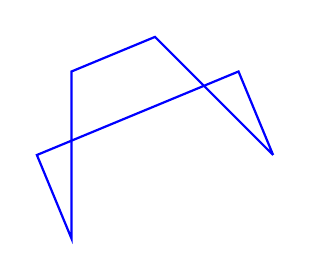
\begin{tikzpicture}[thick,scale=0.5]

	\coordinate (a) at (0:3);
	\coordinate (b) at (45:3); 
	\coordinate (c) at (90:3);
	\coordinate (d) at (135:3);
	\coordinate (e) at (180:3);
	\coordinate (f) at (225:3);
	\coordinate (g) at (270:3);
	\coordinate (h) at (315:3);

	\draw[blue] (a) -- (b) -- (e) -- (f) -- (d) -- (c) -- (a); 
	\draw (a) node {};
	\draw (b) node {};
	\draw (c) node {};
	\draw (d) node {};
	\draw (e) node {};
	\draw (f) node {};
	
\end{tikzpicture}
\hspace{2cm}
		\caption{A graph and the induced RGB graph.}
		\label{rgb}
	\end{center}
	\end{figure}

\subsection{Line Graphs}

 Proximity colorings and $RGB$ graphs become useful to connected matching problems when we consider {\it line graphs}\index{Line graph}.  The line graph of a graph $G$ (denoted $L(G)$) is a graph whose vertex set is the edge set of $G$ and vertices in $L(G)$ are adjacent if and only if the corresponding edges in $G$ share an endpoint. A simple example of a line graph is exhibited in Figure \ref{linegraph}.  
\begin{figure}

	\begin{center}
		\begin{tikzpicture}[thick,scale=0.5]

	\coordinate (a1) at (90:3);
	\coordinate (a2) at (-25:3); 
	\coordinate (a3) at (-155:3);
	\coordinate (a4) at (-90:3);
	\coordinate (a5) at (0:0);

	\draw (a5)-- node [lblvertex] {a}(a1);
	\draw (a5)-- node [lblvertex] {b}(a2);
	\draw (a5)-- node [lblvertex] {c}(a3);
	\draw (a5)-- node [lblvertex] {d}(a4);
	\draw (a3)-- node [lblvertex] {e}(a4);
	\draw (a2)-- node [lblvertex] {f}(a4);

	\draw (a1) node {};
	\draw (a2) node {};
	\draw (a3) node {};
	\draw (a4) node {};
	\draw (a5) node {};
	%\draw (a1) node[lblvertex] {a};
	%\draw (a2) node[lblvertex] {b};  
	
\end{tikzpicture}
\hspace{2cm}
		\begin{tikzpicture}[thick,scale=0.5]

	\coordinate (a) at (90:2.5);
	\coordinate (b) at (25:2.5); 
	\coordinate (c) at (0:0);
	\coordinate (d) at (155:2.5);
	\coordinate (e) at (-55:3);
	\coordinate (f) at (-125:3);

	\draw (a)--(b);
	\draw (b)--(c);
	\draw (c)--(d);
	\draw (d)--(a);
	\draw (a)--(c);
	\draw (c)--(d);
	\draw (b)--(e);
	\draw (e)--(c);
	\draw (d)--(f);
	\draw (f)--(c);
	\draw (d)--(b);
	\draw (e)--(f);
	%\draw (f) arc {-125:-33:3};
	
	\draw (a) node [lblvertex]{a};
	\draw (b) node [lblvertex]{b};
	\draw (c) node [lblvertex]{d};
	\draw (d) node [lblvertex]{c};
	\draw (e) node [lblvertex]{f};
	\draw (f) node [lblvertex]{e};
\end{tikzpicture}
\hspace{2cm}
		\caption{A graph and its line graph.}
		\label{linegraph}
	\end{center}
	\end{figure}

\begin{prop}
Connected matchings in a graph $G$ correspond to green cliques in the RGB graph induced by $L(G)$.  
\end{prop} 

\begin{proof}
	Incident edges of $G$ correspond to adjacent vertices in $L(G)$.  If we have a pair of edges $e, f \in E(G)$ that are disjoint and neighborly, then there is some edge $g \in E(G)$ between an endpoint of $e$ and an endpoint of $f$.  Hence, $eg, fg \in E(L(G))$ and $ef \notin E(L(G))$.  This means that $d_{L(G)}(e,f) = 2$, and $ef$ is green in the RGB graph induced by $L(G)$, as shown in Figure \ref{coresp}.  Since connected matchings are collections of pairwise non-incident and neighborly edges, the green cliques in the RGB graph induced by $L(G)$ correspond to connected matchings in $G$.  
\end{proof}
\begin{figure}
\begin{center}
\begin{tikzpicture}[thick,scale=0.5]

	\coordinate (a0) at (0:0);
	\coordinate (a1) at (180:1);
	\coordinate (a3) at (-109:3);
	\coordinate (a2) at (0:1);
	\coordinate (a4) at (-71:3);
	\coordinate (b1) at (150:3);
	\coordinate (b2) at (30:3);

	\draw (a0)-- node[lblvertex] {a}(a3);
	\draw (a0)-- node[lblvertex] {b}(a4);
	\draw (b1)[blue]--(b2);
	\draw (a0) node {};	
	%\draw (a1) node {};
	%\draw (a2) node {};
	\draw (a3) node {};
	\draw (a4) node {};
	\draw (b1) node[lblvertex, draw = blue] {a};
	\draw (b2) node[lblvertex, draw = blue] {b};
\end{tikzpicture}
\hspace{1cm}
\begin{tikzpicture}[thick,scale=0.5]

	\coordinate (a0) at (0:0);
	\coordinate (a1) at (180:1);
	\coordinate (a3) at (-109:3);
	\coordinate (a2) at (0:1);
	\coordinate (a4) at (-71:3);
	\coordinate (b1) at (150:3);
	\coordinate (b2) at (30:3);

	\draw (a1)-- node[lblvertex] {a}(a3);
	\draw (a2)-- node[lblvertex] {b}(a4);
	\draw (a1)--(a4);
	\draw (b1)[green]--(b2);
	%\draw (a0) node {};	
	\draw (a1) node {};
	\draw (a2) node {};
	\draw (a3) node {};
	\draw (a4) node {};
	\draw (b1) node [lblvertex, draw = green]{a};
	\draw (b2) node [lblvertex, draw = green]{b};
\end{tikzpicture}
\hspace{1cm}
\begin{tikzpicture}[thick,scale=0.5]

	\coordinate (a0) at (0:0);
	\coordinate (a1) at (180:1);
	\coordinate (a3) at (-109:3);
	\coordinate (a2) at (0:1);
	\coordinate (a4) at (-71:3);
	\coordinate (b1) at (150:3);
	\coordinate (b2) at (30:3);

	\draw (a1)-- node[lblvertex] {a}(a3);
	\draw (a2)-- node[lblvertex] {b}(a4);
	%\draw (a1)--(a4);
	\draw (b1)[red]--(b2);
	%\draw (a0) node {};	
	\draw (a1) node {};
	\draw (a2) node {};
	\draw (a3) node {};
	\draw (a4) node {};
	\draw (b1) node[lblvertex, draw = red] {a};
	\draw (b2) node[lblvertex, draw = red] {b};
\end{tikzpicture}

\label{coresp}
\caption{Correspondence between pairs of edges in $G$ and the RGB edges of $L(G)$.}
\end{center}
\end{figure}
Predictably, some complexity results on connected matching problems essentially rest on clique problems in RGB graphs of line graphs.  While clique problems are in general NP hard, there are special classes of graphs, such as perfect graphs, for which they can be solved efficiently.  We will see that some graphs retain this quality in the green graph of their line graph.
 
